\subsection{Internet of Things}
\label{sec:sota_iot}
\subsubsection{Sicherheit}
\label{sec:sota_iot_security}
\subsubsection{Protokolle (BLE, Z-WAVE)}
\label{sec:sota_iot_protocols}
\subsubsection{Smart Home}
\label{sec:sota_iot_smart_home}

\subsection{Smart Locks}
\label{sec:sota_smart_locks}

	relevant: \cite{Ye2017}\cite{Fuller2017}\cite{Rose2016}\cite{Ho2016}
	\missingfigure{Bilder von Smart Lock-Systemen}
	
	\subsubsection{Typische Architekturen und Gemeinsamkeiten}
		\begin{itemize}
			\item Türschloss, häufig elektromagnetisch. Das Öffnen erfolgt primär elektronisch. Alternativ lässt sich das Schluss entweder mit einem Keyfob oder einem physischen Schüssel öffnen.
			\item Mobile Applikation auf einem Smartphone
			\item Herstellereigener Remote Server
		\end{itemize}
		\begin{itemize}
			\item Rollen: Owner, Guest (nur Lock/Unlock)
			\item Permissions: Lock/Unlock, Lock Activity, Guest List, User Invitation (new Users), User Level Control (update User Role), User Permission Control (set time slots for guests)
		\end{itemize}
	
		\begin{figure}[H]
			\centering
			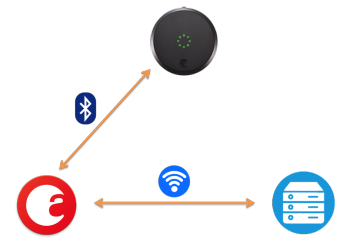
\includegraphics[width=0.5\textwidth]{paperNotes/ye2017_august}
			\caption{Kommunikation zwischen Komponenten des Smart Lock Systems von August}
			\label{fig:august}
		\end{figure}